\documentclass{article}
\PassOptionsToPackage{numbers,compress}{natbib}
\usepackage[final]{template22}
% Common packages
\usepackage[utf8]{inputenc} % allow utf-8 input
\usepackage[T1]{fontenc}    % use 8-bit T1 fonts
\usepackage{microtype}
\usepackage{times}
\usepackage{graphicx}
\usepackage{amsmath,amssymb,mathbbol}
% \usepackage{algorithmic}
% \usepackage[linesnumbered,ruled,vlined]{algorithm2e}
\usepackage{acronym}
\usepackage{enumitem}
\usepackage[pagebackref=true,breaklinks=true,colorlinks]{hyperref}
\usepackage{balance}
\usepackage{xspace}
\usepackage{setspace}
\usepackage[skip=3pt,font=small]{subcaption}
\usepackage[skip=3pt,font=small]{caption}
\usepackage[dvipsnames]{xcolor}
\usepackage[capitalise]{cleveref}
\usepackage{booktabs,tabularx,colortbl,multirow,array,makecell}
% \usepackage{overpic,wrapfig}

\usepackage{fancyhdr}
\hypersetup{pdfencoding=auto,colorlinks=true,allcolors=black}
\renewcommand{\headrulewidth}{0.5pt}
\renewcommand{\footrulewidth}{0pt}
\fancyhf{}
\fancyhead[C]{}
\fancyhead[C]{}
\fancyfoot[C]{\thepage}

% Handy shorthand
\makeatletter
\DeclareRobustCommand\onedot{\futurelet\@let@token\@onedot}
\def\@onedot{\ifx\@let@token.\else.\null\fi\xspace}
\def\eg{\emph{e.g}\onedot} 
\def\Eg{\emph{E.g}\onedot}
\def\ie{\emph{i.e}\onedot} 
\def\Ie{\emph{I.e}\onedot}
\def\cf{\emph{c.f}\onedot} 
\def\Cf{\emph{C.f}\onedot}
\def\etc{\emph{etc}\onedot} 
\def\vs{\emph{vs}\onedot}
\def\wrt{w.r.t\onedot} 
\def\dof{d.o.f\onedot}
\def\etal{\emph{et al}\onedot}
\makeatother

\definecolor{gray}{gray}{0.9}

% Handy math ops
\DeclareMathOperator*{\argmax}{arg\,max}
\DeclareMathOperator*{\argmin}{arg\,min}
\newcommand{\norm}[1]{\left\Vert #1 \right\Vert}

% % Spacing
\frenchspacing
% \medmuskip=2mu   % reduce spacing around binary operators
% \thickmuskip=3mu % reduce spacing around relational operators
% \setlength{\abovedisplayskip}{3pt}
% \setlength{\belowdisplayskip}{3pt}
% \setlength{\abovecaptionskip}{3pt}
% \setlength{\belowcaptionskip}{3pt}
\setlength\floatsep{0.5\baselineskip plus 3pt minus 2pt}
\setlength\textfloatsep{0.5\baselineskip plus 3pt minus 2pt}
\setlength\dbltextfloatsep{0.5\baselineskip plus 3pt minus 2pt}
\setlength\intextsep{0.5\baselineskip plus 3pt minus 2pt}

\makeatletter
\renewcommand{\paragraph}{%
  \@startsection{paragraph}{4}%
  {\z@}{0ex \@plus 0ex \@minus 0ex}{-1em}%
  {\hskip\parindent\normalfont\normalsize\bfseries}%
}
\makeatother

% Graphics path
\graphicspath{{figures/}}

% Clever references
\crefname{algorithm}{Alg.}{Algs.}
\Crefname{algorithm}{Algorithm}{Algorithms}
\crefname{section}{Sec.}{Secs.}
\Crefname{section}{Section}{Sections}
\crefname{table}{Tab.}{Tabs.}
\Crefname{table}{Table}{Tables}
\crefname{figure}{Fig.}{Fig.}
\Crefname{figure}{Figure}{Figure}

% Acronym
\acrodef{pku}[PKU]{Peking University}

\title{Translate books for the visually impaired}

\author{
  Xiang Wang\\
  Department of Artificial intelligence\\
  Peking University\\
  \texttt{2100013146@stu.pku.edu.cn} \\
  \And
  Xin Hao \\
  Department of Artificial intelligence\\
  Peking University\\
  \texttt{2100013152@stu.pku.edu.cn} \\
}

\begin{document}
\maketitle

\begin{abstract}
  The growing spiritual and cultural requirements the blind need to be met. 
  However, barrier-free cultural products take a long time to prepare and are concentrated in more developed cities, they cannot be widespread to those in need. 
  Here we show the pipeline to translate books for the visually impaired mainly with Optical Character Recognition(OCR) and Image Caption(IC) technique. 
  Our work demonstrates how to solve this problem and our result can build the foundation of this task. 
  We anticipate our pipeline to be a starting point of research in translating books for the visually impaired and we hope we can bring light to the blind. 
\end{abstract}

\section{Introduction}
It is consists of four parts: OCR, Image Extractor, Text Typeset and Image Caption. 
Before we feed inputs into the pipeline, we need to preprocess PDF file, turning every page of the PDF file into an image with the same size\footnote{
Actually the same height, because the aspect ratio of one page varies from different books.
}. We call these images as page-images.
OCR module\footnote{
Considering OCR technology is relatively mature, we choose to use existing OCR module. After trying different OCR modules, we choose Paddle OCR because its API is easy to use.
} takes in page-images, and output text boxes, which contains characters and corresponding positions(coordinates). 
Image Extractor also takes in page-images, finds out where the pictures are and cuts out pictures from origin pages. 
With text boxes and positions of pictures, we can typeset the characters into a half-completed book with picture labels in proper place. 
Image Caption module gets pictures from Image Extractor and output descriptions of these pictures. 
Finally, we replace the picture labels with picture descriptions one by one, and output the translated book as .txt file.
\cref{fig:fig1} demonstrates the whole pipeline.

\section{Image Extractor}
This module need to frame every picture in a page with a rectangular area, 
and for a single page, it should output pictures separately and accurately, so that the Image Caption module can produce description for every pictures. 
Of course we can handle this problem with deep learning, but traditional method can work good enough. 
\subsection{Basic idea}

\subsection{Some details}
mask, gray-scale, stride, rectangular

\section{Text Typeset}

\section{Image Caption}


\section{Analyse}


\bibliographystyle{plainnat}
\bibliography{reference}

\appendix

\section{Appendix}
\begin{figure}
    \centering
    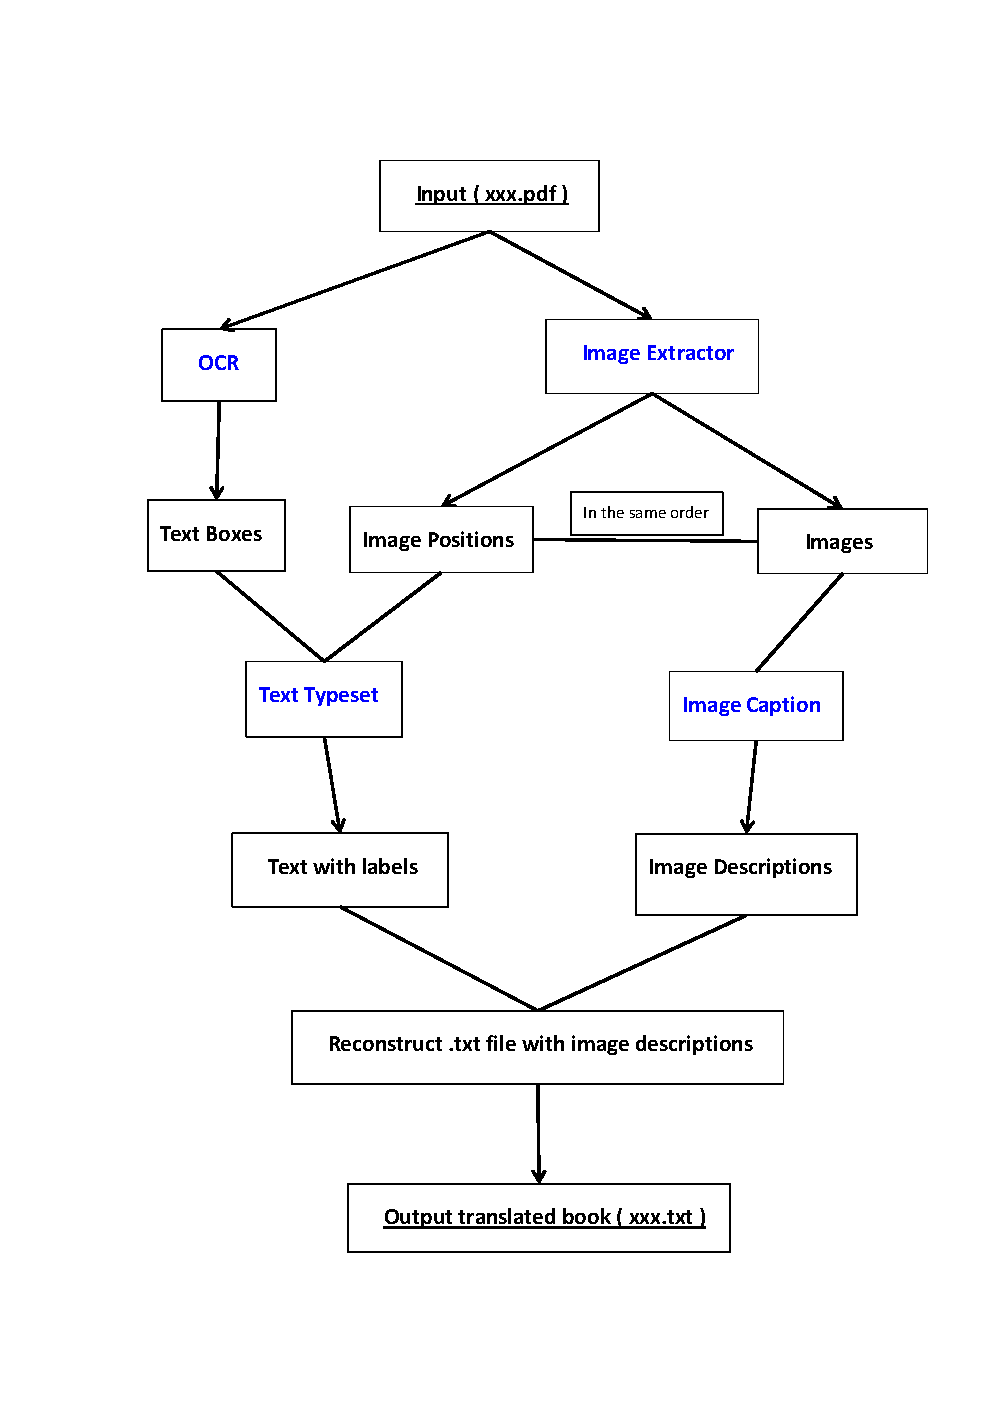
\includegraphics[width=0.8\linewidth]{figures/Overview.png}
    \caption{Pipeline}
    \label{fig:fig1}
\end{figure}

\end{document}